\documentclass{scrartcl}
\usepackage[utf8]{inputenc}
\usepackage[english]{babel}
\usepackage{caption}
\usepackage{subcaption}
\usepackage{listings}
\usepackage{pdfpages}
\usepackage{amsmath,amssymb}
\usepackage{siunitx}
\usepackage{hyperref}
\usepackage{mhchem}
\usepackage[section]{placeins}
\usepackage[activate, protrusion=true, expansion=true]{microtype}
\usepackage[left=2.5cm, right=2.5cm, bottom=2.5cm, top=2.5cm]{geometry}
\usepackage{libertine}
\usepackage{longtable}

\newcommand{\qed}{\hfill $\blacksquare$}
\newcommand{\gitlab}{\href{https://gitlab.lrz.de/arne/neuroprosthetics}{GitLab}}

\lstset{frame=single,keepspaces=true,captionpos=b}

\title{Digital 3D Geometry Processing}
\subtitle{Exercise 3}
\author{\textsc{Niklas Schmitz} \and \textsc{Jannik Reichert} \and \textsc{Arne Sachtler}}
\date{\today}

\begin{document}
\maketitle

\section{Signed Distance Function for a Line}
The line $x = y$ is given and the signed distance function is sought.
We consider the line as being a degenerated circle with infinite radius, that is, the line has an inside and an outside.
Then we get the following signed distance function
\begin{equation}
	\Phi (x,y) = \sqrt{\frac{1}{2}} (y - x) \, .
\end{equation}

\section{Curve with Sharp Corner}

Consider the following curve
\begin{equation}
	\begin{pmatrix}x\\y\end{pmatrix} = \begin{pmatrix}t^2 (t-1) (t+1)\\t (t-1) (t+1)\end{pmatrix} \text{ for } t \in [0, 1]\, .
\end{equation}
This parametric curve has the shape shown in Figure~\ref{fig:disc}. The discontinuity of this shape is at the origin.
\begin{figure}[h]
	\centering
	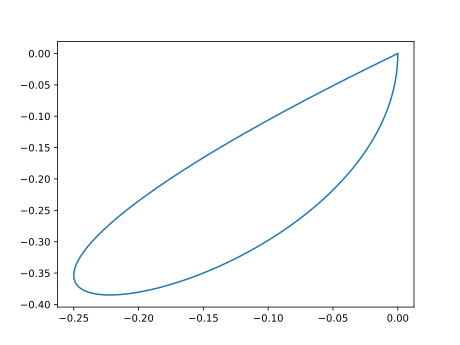
\includegraphics[height=5cm]{figures/discontinuous_curve.pdf}
	\caption{Discontinous curve where the components are governed by continuous polynomials.}
	\label{fig:disc}
\end{figure}



\section{Does the Chord Length Always Converge?}

\section{A Sequence of 2D Curves}
	
\end{document}
